%%%% PREAMBLE %%%%%%%%%%%%%%%%%%%%%%%%%%%%%%%%%%%%%%%%%%%%%%%%%%%%%%%%%%%%%%%%%%%%%%%%%%%%%%%%%%%%%

\documentclass[a4paper,12pt]{article}

\usepackage{Packages}


\begin{document}

%%%% TITLE & ABSTRACT %%%%%%%%%%%%%%%%%%%%%%%%%%%%%%%%%%%%%%%%%%%%%%%%%%%%%%%%%%%%%%%%%%%%%%%%%%%%%

~\\[3.5cm]

\begin{center}

{\huge \bfseries
    Title
}\\[0.5cm]

\textbf{Author Name - Affiliation - Email}\\[2.5cm]


\begin{abstract}
{\it
    Nice abstract.

    With amazingly clear and concise paper description.

    Compilation date at the bottom of the page if required.
}
\end{abstract}

\end{center}


\vfill
\centerline{\large \today}



%%%% TABLE OF CONTENTS %%%%%%%%%%%%%%%%%%%%%%%%%%%%%%%%%%%%%%%%%%%%%%%%%%%%%%%%%%%%%%%%%%%%%%%%%%%%

\newpage
\tableofcontents
\newpage



%%%% SECTIONS OR CHAPTERS %%%%%%%%%%%%%%%%%%%%%%%%%%%%%%%%%%%%%%%%%%%%%%%%%%%%%%%%%%%%%%%%%%%%%%%%%

\section*{Introduction}
\label{sec:Intro}
\addcontentsline{toc}{section}{Introduction}
\markboth{Introduction}{}

{\it
\textbf{Note:} Throughout this report, if a term is Capitalised, then its definition (or a closely related one) is
generally found either in the main body or in Appendix \ref{sec:BasicDefs} \\
}

Equally clear introduction.
Here are a couple of glossary entries: \gls{QM} and \gls{QI}.
And a reference to a section: Appendix \ref{sec:CoreMathsOfQM}.




% \input for no pagebreak, \include for pagebreak

\section{Background Theory}
\label{sec:BackgroundTheory}



\subsection{Quantum Mechanics and Information}
\label{sec:SubQMandInfo}

A long acronym entry: \acrlong{QI}.
Author and Year Citations: \citeauthor{Shannon1948} in \citeyear{Shannon1948}.
A definition with mathematical expressions:\\


The conventional system used in \gls{QI} is the \gls{QM} analogue to the Bit:
\begin{defn}\label{def:Q_Reg}
    A \textbf{Quantum Bit} (or \textbf{Qubit}) is a quantum system with basis $B = \{|0\rangle,|1\rangle\}$, whose states $|\psi\rangle$ are therefore of the form
    $$
        |\psi\rangle = \alpha_{0}|0\rangle + \alpha_{1}|1\rangle \, \in \mathcal{H}_{\{0,1\}}, \quad \text{where} \quad
        \alpha_{0}, \alpha_{1} \in \mathbb{C}_{1} \; \big| \; |\alpha_{0}|^{2} + |\alpha_{1}|^{2} = 1
    $$
    A set of qubits is called a \textbf{Quantum Register}; for an $n$-qubit register the state space is then
    $$
        \mathcal{H}_{\{0,1\}^{n}} = \bigotimes_{i=1}^{n} \mathcal{H}_{\{0,1\}} = \mathcal{H}_{\{0,1\}}^{[n]}
    $$
\end{defn}


\begin{equation}\label{eq:CompositeInclusions}
    B^{n} \, \subsetneq \,
    \mathcal{H}_{B}^{n} \, \subsetneq \,
    \mathcal{H}_{B}^{[n]} = \mathcal{H}_{B^{n}}
\end{equation}



\subsection{Visualising Qubit States}
\label{sec:SubVisualStates}

A minipage to show an image beside a column of text:\\

\begin{minipage}{0.5\textwidth} \centering
    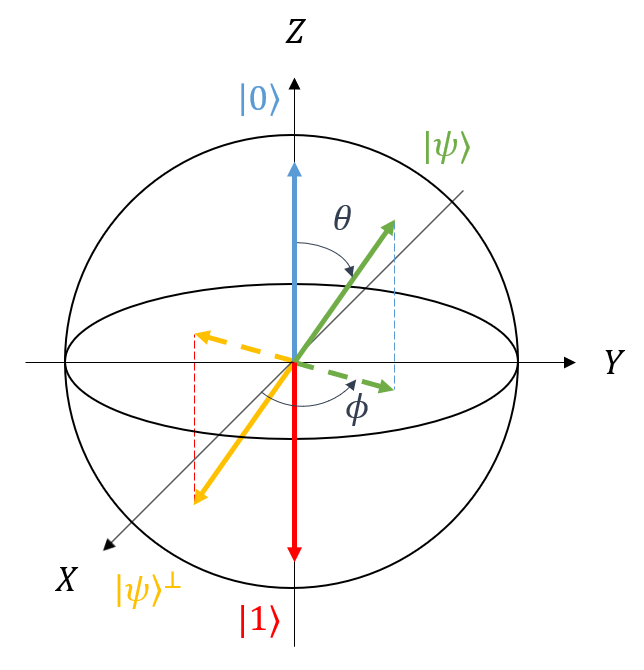
\includegraphics[width=9cm]{BlochSphere}
    \captionof{figure}{\it Bloch Sphere}
    \label{fig:BlochSphere}
\end{minipage}
\begin{minipage}{0.5\textwidth}

Qubit (Pure) States can be visualised on the Bloch Sphere, a unitary sphere in 3D Space, with the standard parametrisation:
$$
    |\psi\rangle = \cos\left(\frac{\theta}{2}\right) |0\rangle + e^{i\phi} \sin\left(\frac{\theta}{2}\right) |1\rangle
$$
Consequently, a Mixture of States can be visualised as a set of vectors on the Bloch Sphere, each associated with a (classical)
probability weighting.\\

A noteworthy feature of the Bloch Sphere is that unlike in standard 3D space, Orthogonality is not given by states $\pi/2$ from
the given one; it is instead given by the (unique) \underline{opposite} state;
it is easy to see that the inner product of opposite states is 0:
\begin{equation}\label{eq:OrthState}
    \alpha |0\rangle + \beta |1\rangle \quad \perp \quad \beta^{*} |0\rangle - \alpha^{*} |1\rangle
\end{equation}

\end{minipage}\\[0.5cm]



\subsection{Entanglement}
\label{sec:SubEntanglement}

An Example:

\begin{exmp}\label{ex:Entanglement}
    In this 3-qubit-system state $|\psi\rangle$, qubits A and B are entangled with each other while in a product state with qubit C:
    \begin{align*}
        |\psi\rangle & = \frac{1}{2\sqrt{2}} (|000\rangle + |010\rangle - |100\rangle + |110\rangle + |001\rangle + |011\rangle - |101\rangle + |111\rangle) \\
                    & = \frac{1}{2\sqrt{2}} (|00\rangle_{AB} + |01\rangle_{AB} - |10\rangle_{AB} + |11\rangle_{AB}) \otimes (|0\rangle_{C} + |1\rangle_{C})
    \end{align*}
    Furthermore, in this case it is not possible to detect the entanglement by just analysing measurement probabilities since they depend on the
    modulus of coefficients, making them equal to those for the state with no $-$ signs.
\end{exmp}



\section{Measurement \& State Discrimination}
\label{sec:MeasurAndStateDiscr}


\subsection{Measurement Classes}
\label{sec:SubPOVMclasses}

A textwidth-wide Figure and a reference to it: Figure \ref{fig:POVMclasses}.

\begin{figure}\centering
    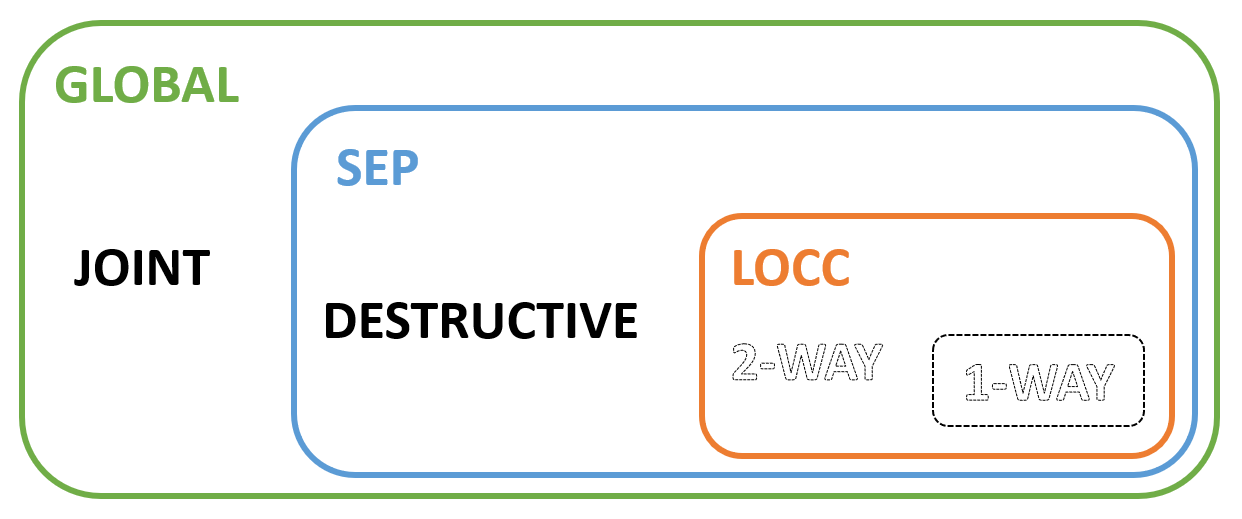
\includegraphics[width=\textwidth]{POVMclasses}
    \caption{\it POVM Classes' Containment}
    \label{fig:POVMclasses}
\end{figure}



\section{Libraries}
\label{sec:Libraries}

This section is here to showcase the listings environment varieties:
inline, as item label in a description environment and as a stand-alone listing. 



\subsection{GSM}
\label{sec:Sub_GSM}

The \acrlong{GSM} library \cite{GSM} implements a computational construct similar to a Turing Machine over a graph,
where states are node combinations (though more information may be stored) and where the arbitrary transition function
can update both state and graph.

\begin{defn}\label{def:GSM}
Given a \lstinline{Graph} with typed nodes and a \lstinline{State} object of arbitrary structure,
a \textbf{\gls{GSM}} is defined by the functions it applies to perform a step:
\begin{description}[noitemsep]
    \lstitem{Selector} A function to extract a list of nodes from the arbitrarily-structured \lstinline{State} 
    \lstitem{Scanner} A generalised neighbourhood function, which scans the graph ``around'' the state nodes, 
            optionally applying some filter (e.g. node type), and returns a scored list of nodes for further processing
    \lstitem{Updater} A function to process the scan result and thus update the state and/or the graph itself
\end{description}
\end{defn}



\subsection{GPy-ABCD}
\label{sec:Sub_GPyABCD}

A full listing, which has a label, a caption and language-aware highlighting.

\begin{lstlisting}[label=lst:GPyABCD_function, language=Python, caption=Main GPy-ABCD \cite{GPy_ABCD} model-space search function with default arguments, breaklines=true, basicstyle=\ttfamily\small]
    import numpy as np
    from GPy_ABCD import *


    if __name__ == '__main__':
        # Example data
        X = np.linspace(-10, 10, 101)[:, None]
        Y = np.cos((X - 5) / 2) ** 2 * X * 2 + np.random.randn(101, 1)

        # Main function call with default arguments
        best_mods, all_mods, all_exprs, expanded, not_expanded = explore_model_space(X, Y,
            start_kernels = start_kernels['Default'], p_rules = production_rules['Default'],
            utility_function = BIC, rounds = 2, beam = [3, 2, 1], restarts = 5,
            model_list_fitter = fit_mods_parallel_processes, optimiser = GPy_optimisers[0],
            verbose = True)

        print('\nFull lists of models by round:')
        for mod_depth in all_mods: print(', '.join([str(mod.kernel_expression) for mod in mod_depth]) + f'\n{len(mod_depth)}')

        print('\n\nTop-3 models\' details:')
        for bm in best_mods[:3]:
            model_printout(bm) # See the definition of this convenience function for examples of model details' extraction
            print('Prediction at X = 11:', bm.predict(np.array([11])[:, None]), '\n')

        from matplotlib import pyplot as plt
        plt.show()
\end{lstlisting}




%\newpage
\section*{Conclusion}
\label{sec:Conclusion}
\addcontentsline{toc}{section}{Conclusion}
\markboth{Conclusion}{}

Great conclusion to finish things off.






%%%% APPENDICES AND BIBLIOGRAPHY %%%%%%%%%%%%%%%%%%%%%%%%%%%%%%%%%%%%%%%%%%%%%%%%%%%%%%%%%%%%%%%%%%

% References here or below
\addcontentsline{toc}{section}{References}
\markboth{Conclusion}{}
\printbibliography

%\newpage

\appendix

\section{Acronyms}
\label{sec:Acronyms}

\printacronyms

\section{Basic Definitions}
\label{sec:BasicDefs}

\printglossary


% Other Appendices

\section{Core Mathematics of Quantum Mechanics}
\label{sec:CoreMathsOfQM}



\subsection{Mathematical Bases}
\label{sec:SubMathBases}

The content of this appendix only serves to showcase a missing reference, how Appendix references are shown and simple lists.\\

As will be made clear shortly (in Definition \ref{def:QMPostulates}), it is specifically \gls{Unitary} Hilbert Spaces which are of concern to \gls{QM},
and the common notation in treating them is different from the standard mathematical one used for Inner Product Space:

\begin{defn}\label{def:DiracNotation}
    The \textbf{Dirac Notation} (or \textbf{Bra-Ket Notation}) is the following:
    \begin{itemize}[noitemsep]
        \item Vectors are denoted $|v\rangle$ (``Ket'')
        \item Covectors (vectors of the \gls{Dual Space}) are denoted $\langle v|$ (``Bra'')
        \item Inner Products are denoted $\langle\cdot|\cdot\rangle$ (``Bra-(c)-Ket''), where \textbf{linearity is swapped} with respect to standard notation:
            here it is the second term which is linear, while the first is conjugate-linear
        \item Outer Products are denoted $|\cdot\rangle\langle\cdot|$ (for matching `Ket' and `Bra' this is simply a projector operator)
    \end{itemize}
    The fact that `Bra's $\langle\psi|$ are precisely the Dual Vectors of `Ket's $|\psi\rangle$ is the key to the usefulness of this notation:
    \begin{itemize}[noitemsep]
        \item The relation between the two is the very elegant one of \glspl{Hermitian Conjugate}: $\langle\psi| = |\psi\rangle^{\dagger}$
        \item Making the `Bra's interpretable as linear functions on Kets justifies the notation for the Inner Product: $\langle v| \cdot |w\rangle$ is indeed
            equivalent to $\langle v|w \rangle$ (which is equal to $\langle |w\rangle,|v\rangle \rangle$ in standard Inner Product notation with Ket notation vectors)
    \end{itemize}
\end{defn}




%\newpage

\section{Detailed Calculations}
\label{sec:DetailedCalculations}

An appendix for skipped calculation details, showcasing the tedious LaTeXing of matrices.
This section contains the main orthogonal pair system's calculation details skipped in Section \ref{sec:ProjectWork}.



\subsection{Total System Density}
\label{sec:SubTotSymDens}

Some Matrices:
\begin{equation}\label{eq:Diagonalisation}
    \hat{\rho} =    \frac{1}{6}
                    \begin{pmatrix}
                        1 &  0 &  0 & 0 \\
                        0 &  2 & -1 & 0 \\
                        0 & -1 &  2 & 0 \\
                        0 &  0 &  0 & 1
                    \end{pmatrix}
               =    EDE^{-1}, \; \text{where} \;
    D = \frac{1}{6}
        \begin{pmatrix}
            1 & 0 & 0 & 0 \\
            0 & 1 & 0 & 0 \\
            0 & 0 & 3 & 0 \\
            0 & 0 & 0 & 1
        \end{pmatrix} \; \text{and} \;
    E = \begin{pmatrix}
            1 &  0 &  0 & 0 \\
            0 & \frac{1}{\sqrt{2}} &  \frac{1}{\sqrt{2}} & 0 \\
            0 & \frac{1}{\sqrt{2}} & -\frac{1}{\sqrt{2}} & 0 \\
            0 &  0 &  0 & 1
        \end{pmatrix} = E^{-1}
\end{equation}




%\newpage

\begin{comment}
% References here or above
\addcontentsline{toc}{section}{References}
\markboth{Conclusion}{}
\printbibliography
\end{comment}



%%%%%%%%%%%%%%%%%%%%%%%%%%%%%%%%%%%%%%%%%%%%%%%%%%%%%%%%%%%%%%%%%%%%%%%%%%%%%%%%%%%%%%%%%%%%%%%%%%%

\end{document}